% Just The Docs Front Matter
% title: Sea-Level Fingerprints (GRACE)
% parent: Tutorials
% has_children: false
% has_toc: false

\subsection{Sea-Level Fingerprints (GRACE)} \label{sec:using-issm-tutorials-sealevelfingerprints}
\subsubsection{Goals} %{{{
\begin{itemize}
	\item Setup a ISSM-SESAW model with GRACE-based forcing
	\item Run the model to compute sea-level fingerprints
\end{itemize}

Go to \lstinlinebg|<ISSM_DIR>/examples/SlrGRACE/| to do this tutorial.

%}}}
\subsubsection{Mesh} %{{{
Set \lstinlinebg|steps = 1| to create an unstructured global mesh. Choose \lstinlinebg|mindistance_coast|, \lstinlinebg|mindistance_lan|, and \lstinlinebg|maxdistance| as you wish for generating a mesh. The nominal parameters should generate the following mesh:
\begin{figure}[H]
	\begin{center}
		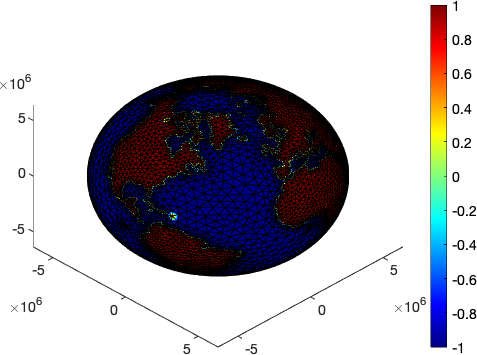
\includegraphics[width=\textwidth]{\assetsParentPath/assets/img/using-issm/tutorials/sealevelfingerprints/Mesh.png}
	\end{center}
\end{figure}
%}}}
\subsubsection{GRACE loads} %{{{
Set \lstinlinebg|steps = 2| to load GRACE-based estimate of water equivalent height (WEH) change for a chosen month. Choose \lstinlinebg|year_month| as you wish. The nominal month is January 2007 and here is the load model (cf. \lstinlinebg|steps = 5| for plotting):
\begin{figure}[H]
	\begin{center}
		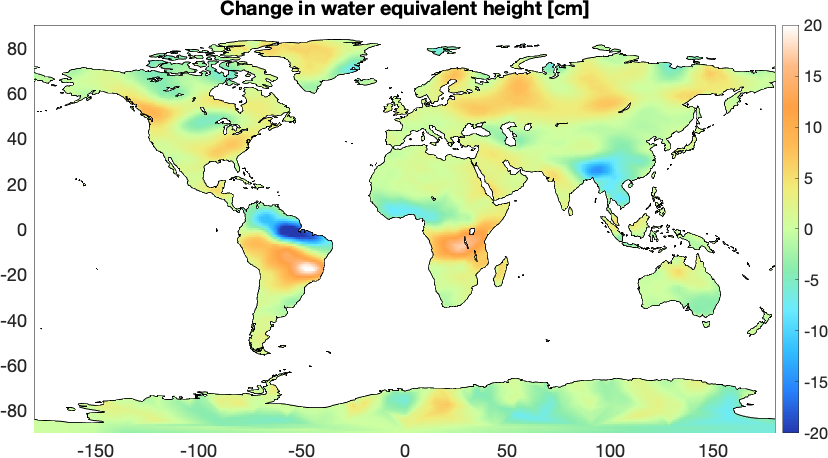
\includegraphics[width=\textwidth]{\assetsParentPath/assets/img/using-issm/tutorials/sealevelfingerprints/Weh.png}
	\end{center}
\end{figure}
%}}}
\subsubsection{Parameterization} %{{{
In the next step, you will load the Earth model. The nominal model is PREM; \lstinlinebg|lovenumbers| reads the associated Love numbers. You will also have to set up some standard parameters regarding ice sheets for passing the consistency.
%}}}
\subsubsection{Solve Model} %{{{
In \lstinlinebg|steps = 4|, you will choose the solid-Earth physics (e.g., gravitation, viscoelasticity, and rotation) that you wish to consider. You may also request model outputs (e.g., sea level and bedrock motion). You must set \lstinlinebg|masstransport| and \lstinlinebg|slc| flags on before solving the \lstinlinebg|transient| model. See \lstinlinebg|steps = 6| for running a model with multiple (transient) loads.
%}}}
\subsubsection{Some Results} %{{{
Once the model run is completed, you may plot results. Some useful plotting scripts are located in \lstinlinebg|steps = 5| and \lstinlinebg|steps = 7|. In the latter, you can also find a script to make an animation. Here is an example result for January 2007:
\begin{figure}[H]
	\begin{center}
		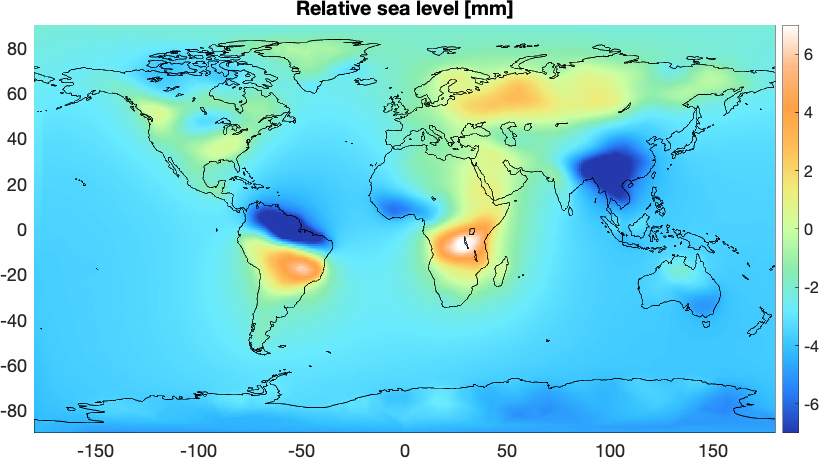
\includegraphics[width=\textwidth]{\assetsParentPath/assets/img/using-issm/tutorials/sealevelfingerprints/Rsl.png}
	\end{center}
\end{figure}
%}}}

\clearpage % Make sure all figures are placed before next section
